\documentclass{article}
\usepackage[polish]{babel}
\usepackage{minted}
\usepackage[letterpaper,top=2cm,bottom=2cm,left=3cm,right=3cm,marginparwidth=1.75cm]{geometry}
\usepackage{amsmath}
\usepackage{graphicx}
\usepackage[colorlinks=true, allcolors=blue]{hyperref}
\usepackage[T1]{fontenc}
\usepackage[table,xcdraw]{xcolor}
\usepackage{float}
\usepackage[figurename=Wykres]{caption}

\title{MOwNiT - Funkcje sklejane}
\author{Jakub Frączek}

\begin{document}

\maketitle

\section{Temat ćwiczenia}

Dla funkcji f(x) zadanej w zadaniu dotyczącym interpolacji wyznaczyć interpolacyjną funkcję 
sklejaną trzeciego stopnia oraz drugiego stopnia. Dla obu rodzajów funkcji (2-go i 3-go 
stopnia) należy wykonać obliczenia dla co najmniej dwóch różnych warunków brzegowych.  
Podobnie jak poprzednio określić dokładność interpolacji – dla różnej liczby przedziałów i 
dla różnych warunków brzegowych.  
Porównać interpolację funkcjami sklejanymi drugiego i trzeciego stopnia. Graficznie 
zilustrować interesujące przypadki.  
Opisać dokładnie przyjęte warunki brzegowe. 

\section{Funkcja dla której przeprowadzone zostało doświadczenie}

\begin{center}
\(f(x) = 10 * m + \frac{\mathrm{x}_{}^{2}}{k} - 10 * m * cos(k*x)\)
\end{center}

\noindent
gdzie:

\bigbreak

\(k = 1.5\)
\newline \indent
\(m = 3.0\)
\newline \indent
\(x \in [-4\pi, 4\pi]\)
\bigbreak
Wykres funkcji (wykres 1)

\begin{figure}[H]
  \centering
  \begin{minipage}[b]{0.4\textwidth}
    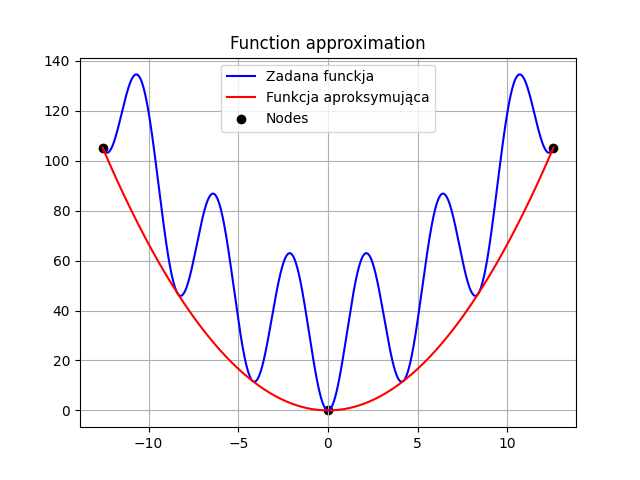
\includegraphics[width=\textwidth]{img01.png}
    \caption{Dana funkcja}
  \end{minipage}
\end{figure}

\section{Dane techniczne}

\subsection{Hardware}

Laptop z procesorem Intel Core i5-9300H 2.4GHz oraz 32 GB pamięci RAM.

\subsection{Software}

Wykorzystany został system Windows 11 x64 oraz język Python w wersji 3.11.8 wraz z bibliotekami:
\begin{itemize}
\item math
\item copy
\item matplotlib
\item numpy
\end{itemize}

\section{Funkcje sklejane}

\subsection{Kwadratowa funkcja sklejana}

\subsubsection{Wyznaczanie współczynników}

Kwadratowa funkcja sklejona musi spełniać warunki:

\begin{itemize}
    \item \( S_i (x) = a_i + b_i(x - x_i) + c_i(x - x_i)^2\) \ (1)
    \item \(S_i(x_i) = f(x_i) = y_i\) (2)
    \item \(s_i(\mathrm{x}_{i+1}^{}) = S_{i + 1}(x_{i+1})\) \ (3)
    \item \(S'_i(x_{i+1}) = S'_{i+1}(x_{i+1})\) \ (4)
\end{itemize}

\noindent
Podstawiam \(x_i\) do (1) i korzystam z właności (2), z tego otrzymuję:

\[y_i = S_i (x_i) = a_i + b_i(x_i - x_i) + c_i(x_i - x_i)^2 = a_i \Rightarrow  a_i = y_i \ \ (5)\] 
\noindent
Korzystając z warunku (1) i (4):

\[b_{i+1} + 2c_{i+1}(x_{i+1}-x_{i+1}) = b_i + 2c_i(x_{i+1} - x_i)\]

\[b_{i+1} = b_i + 2c_i(x_{i+1} - x_i)\]

\[c_i = \frac{b_{i+1}-b_i}{2(x_{i+1}-x_i)} \ \ (6)\] 
\noindent
Korzystając z (1), (2), (3) i (5):

\[y_{i+1} = S_i(x_{i+1}) = S_{i+1}(x_{i+1}) = y_i + b_i(x_{i+1} - x_i) + c_i(x_{i+1}-x_i)^2 \ \ (7)\]
\noindent
Korzystając z (6) i (7):

\[y_{i+1} - y_i = b_i(x_{i+1}-x_i) + \frac{b_{i+1}-b_i}{2(x_{i+1}-x_i)}(x_{i+1}-x_i)^2\]

\[\frac{y_{i+1} - y_i}{x_{i+1}-x_i} = b_i + \frac{1}{2}b_{i+1} - \frac{1}{2}b_i\]

\[2\cdot \frac{y_{i+1} - y_i}{x_{i+1}-x_i} = b_{i+1}+b_i\]

\[b_i + b_{i-1} = 2\frac{y_i - y_{i-1}}{x_i - x_{i-1}}\]
\noindent
Oznaczam \(\frac{y_i - y_{i-1}}{x_i - x_{i-1}}\) jako \(v\) i tworzę układ równań w celu wyliczenia
wspołczynnika \(b_i\)

\bigbreak

\[b_1 + b_2 = 2v_2\]
\[b_2 + b_3 = 2v_3\]
\[\vdots\]
\[b_{n-2}+b_{n-1}=2v_{n-1}\]

\begin{gather*}
\begin{bmatrix}
1 & 1 & 0 & \cdots & 0 \\
0 & 1 & 1 & \ddots & \vdots \\
\vdots & \ddots & \ddots & \ddots & 0 \\
0 & \cdots & 0 & 1 & 1 
\end{bmatrix}  
\begin{bmatrix}
b_1 \\
b_2 \\
\vdots \\
b_{n-1} 
\end{bmatrix} 
=
\begin{bmatrix}
2v_1 \\
2v_2 \\
\vdots \\
2v_{n-1} 
\end{bmatrix}
\end{gather*}
\noindent
Jak widać jest n - 1 równań i n niewiadowmych, zatem trzeba będzie ustalić doddatkowy warunek brzegowy.

\subsubsection{Natural Boundary}

Założenia:

\[S'_1(x_1) = 0 \ \ \vee \ \ S'_{n-1}(x_n) = 0 \ \ (8)\]
\noindent
Korzystając z (1) i (8):

\[S'_1(x_1) = 0 = b_1 + 2c_1(x_1-x_1) \Rightarrow b_1 = 0 \ \ (9)\]
\noindent
Zatem:

\[b_1+b_2 = 2v_2 \Rightarrow b_2 = 2v_2\]

\[b_2 + b_3 = 2v_3 \Rightarrow b_3 = 2v_3-2v_2\]

\[\vdots\]

\[b_n = 2(v_n-v_{n-1}+v_{n-2}-...\pm v_2)\]

\subsubsection{Clamped Boundary}
\noindent
Założenia:

\[S'_1(x_1) = f'_1(x) \ \ \vee \ \ S'_{n-1}(x_n) = f'_{n-1}(x) \ \ (10)\]
\noindent
\(f'_1(x)\) można zapisać jako:
\[f'_1(x) = \frac{y_2-y_1}{x_2-x_1} \ \ (11)\]
\noindent
Korzystając z (1), (10) i (11):

\[b_1 + 2c_1(x_1 - x_1) = \frac{y_2 - y_1}{x_2-x_1} \Rightarrow  b_1 = \frac{y_2 - y_1}{x_2-x_1} = v_2\]

\bigbreak
\noindent
Zatem:

\[b_1 + b_2 = 2v_2 \Rightarrow b_2 = v_2\]

\[b_2 + b_3 = 2v_3 \Rightarrow b_3 = 2v_3 - v_2 \]

\[\vdots \]

\[b_n = 2(v_n-v_{n-1}+v_{n-2}+...\pm v_3) \pm v_2\]

\subsection{Sześcienna funkcja sklejana}

\subsubsection{Wyznaczanie współczynników}

Wzór na sześcienną funkcję sklejaną został podany poniżej:

\[s(x) = \mathrm{a}_{i}^{} + \mathrm{b}_{i}^{}\cdot (x - \mathrm{x}_{i}^{}) +\mathrm{c}_{i}^{}\cdot \mathrm{(x - \mathrm{x}_{i}^{})}_{}^{2} + \mathrm{d}_{i}^{}\cdot  \mathrm{(x-\mathrm{x}_{i}^{})}_{}^{3} \ dla \ x \in [\mathrm{x}_{i}^{}, \mathrm{x}_{i + 1}^{}]\]
\noindent
Dodatkowo funkcja sklejana 3-go stopnia musi spełniać poniższe warunki:
\begin{itemize}
\item \(S_i(x_{i+1}) = f(x_{i+1})\)
\item \(S_i(x_{i+1}) = S_{i+1}(x_{i+1})\)
\item \(S'i(x_{i+1}) = S'_{i+1}(x_{i+1})\)
\item \(S''(x_{i+1}) = S''_{i+1}(x_{i+1})\)
\end{itemize}
\noindent
Ponieważ \(S_i(x)\) jest sześcienna, to \(S''_i(x)\) jest liniowa na przedziale \([x_i, x_{i+1}]\). Wprowadzam \(h_i = x_{i+1} - x_i\), wtedy:

\[S''_i(x) = S''_i(x_i)\frac{x_{i+1}-x}{h_i} + s''_i(x_{i+1})\frac{x-x_i}{h_i}\]
\noindent
Całkując dwukrotnie otrzymuję:

\[S_i(x) = \frac{S''_i(x_i)}{6h_i}(x_{i+1}-x)^3 + \frac{S''_i(x_{i+1})}{6h_i}(x-x_i)^3+C(x-x_i)+D(x_{i+1}-x)\],
\noindent
gdzie C i D - stałe całkowania
\noindent
Korzystając z warunków interpolacji:
\noindent
\(S_i(x_i) = y_i\) oraz \(S_i(x_{i+1}) = y_{i+1}\) można wyliczyć C i D. Po wyliczeniu tych stałych otrzymujemy:

\[S_i(x) = \frac{S''_i(x_i)}{6h_i}(x_{i+1}-x)^3 + \frac{S''_i(x_{i+1})}{6h_i}(x-x_i)^3 + 
(\frac{y_{i+1}}{h_i} - \frac{S''_i(x_{i+1})h_i}{6})(x-x_i) + (\frac{y_i}{h_i}-\frac{S''_i(x_i)h_i}{6})(x_{i+1}-x)\]
\noindent
W powyższym wzorze nadal nie znamy \(S''_i(x)\). W celu jego wyliczenia należy skorzystać z warunku ciągłości pierwszech pochodnej. Różniczkuję zatem \(S_i(x)\):

\[S'_i(x_i) = -\frac{h_i}{3}S''_i(x_i) - \frac{h_i}{6}S''_i(x_{i+1}) - \frac{y_i}{h_i} + \frac{y_{i+1}}{h_i}\]
\noindent
Dla przejrzystości należy wprowadzić dwa symbole:
\begin{itemize}
\item \(\sigma_i = \frac{1}{6}S''(x_i)\)
\item \(\Delta_i = \frac{y_{i+1}-y_i}{h_i}\)
\end{itemize}
\noindent
Wtedy:

\[S'_i(x_i) = -2\sigma_ih_i - \sigma_{i+1}h_i + \Delta_i\]
\[S'_i(x_i) = \Delta_i - h_i(\sigma_{i+1}+2\sigma_i)\]
\noindent
Wtedy:

\[S'_{i-1}(x_i) = \Delta_{i-1} + h_{i-1}(2\sigma_i + \sigma_{i-1})\]
\noindent
Teraz korzystając z warunku ciągłości (\(S'_{i-1}(x_i) = S'_i(x_i)\)):

\[\Delta_{i-1} + h_{i-1}(2\sigma_i + \sigma_{i-1}) = \Delta_i - h_i(\sigma_{i+1} + 2\sigma_i)\]
\noindent
Finalnie otrzymujemy układ równań liniowych:

\[h_{i-1}\sigma_{i-1} + 2(h_{i-1}+h_i)\sigma_i + h_i\sigma_{i+1} = \Delta_i - \Delta_{i-1}, i = 2,3,...,n-1\]
\noindent
Jak można zauważyć w układzie równań mamy n niewiadomych i n - 2 równań, zatem należy określić dwa dodatkowe warunki brzegowe.

\subsubsection{Default Boundary}

Warunki:

\begin{itemize}
\item \(C_1(x)\) - f. sześcienna przez pierwsze 4 punkty
\item \(C_n(x)\) - f. sześcienna przez ostatnie 4 punkty
\end{itemize}

\[S'''(x_1) = C'''_1 \ \ \ S'''(x_n) = C'''_n\]
\noindent
Stałe \(C'''_1 i C'''_n\) mogą być określone bez znajomości \(C_1(x)\) i \(C_n(x)\):

\begin{itemize}
\item \(\Delta_i^{(1)} = \frac{y_{i+1} - y_i}{x_{i+1}-x_i}\)
\item \(\Delta_i^{(2)} = \frac{\Delta_{i+1}^{(1)}-\Delta_i^{(1)}}{x_{i+2}-x_i}\)
\item \(\Delta_i^{(3)} = \frac{\Delta_{i+1}^{(2)}-\Delta_i^{(2)}}{x_{i+3}-x_i}\)
\end{itemize}
\noindent
Różniczkując wzór na \(S''(x)\) na przedziale \([x_i, x_{i+1}]\), otrzymujemy:

\[S'''(x_1) = C'''_1(x_1) \Rightarrow  \frac{6}{h_1}(\sigma_2-\sigma_1) = 6\Delta_i^{(3)}\]

\[S'''(x_n) = C'''_n(x_n) \Rightarrow  \frac{6}{h_{n-1}}(\sigma_n - \sigma_{n-1}) = 6\Delta_{n-3}^{(3)}\]
\noindent
Po przekształceniu otrzymujemy:

\begin{itemize}
\item \(-h_1\sigma_1 + h_1\sigma_2 = h_1^2\Delta_1^{(3)}\)
\item \(h_{n-1}\sigma_{n-1} - h_{n-1}\sigma_n = -h_{n-1}^2\Delta_{n-3}^{(3)}\)
\end{itemize}
\noindent
Finalnie otrzymujemy:

\begin{gather*}
\begin{bmatrix}
-h_1 & h_1 & 0 & 0 & 0 \\
h_1 & 2(h_1+h_2) & h_2 & 0 & 0 \\
0 & h_2 & 2(h_2+h_3) & h_3 & 0 \\
\vdots & \vdots & \vdots & \vdots & \vdots \\
0 & 0 & h_{n-2} & 2(h_{n-2} + h_{n-1}) & h_{n-1} \\
0 & 0 & 0 & h_{n-1} & -h_{n-1} 
\end{bmatrix}
\begin{bmatrix}
\sigma_1 \\
\sigma_2 \\
\sigma_3 \\
\vdots \\
\sigma_{n-1} \\
\sigma_n 
\end{bmatrix}
=
\begin{bmatrix}
\mathrm{h}_{1}^{2}\mathrm{\Delta}_{1}^{(3)} \\
\Delta_2 - \Delta_1 \\
\Delta_3 - \Delta_2 \\
\vdots \\
\mathrm{\Delta}_{n-1}^{} - \mathrm{\Delta}_{n-2}^{} \\
\mathrm{-h}_{n-1}^{2}\mathrm{\Delta}_{n-3}^{(3)} 
\end{bmatrix}
\end{gather*}

\subsubsection{Natural Boundary}

Warunki:

\[S''(x_1) = S''(x_n) = 0\]
\noindent
Biorąc pod uwagę, że \(\sigma_i = \frac{1}{6}S''_i(x_i)\) otrzymujemy:

\[S''(x_1) = S''_1(x_1) = 0 \Leftrightarrow \sigma_1 = 0\]

\[S''(x_n) = S''_n(x_n) = 0 \Leftrightarrow \sigma_n = 0\]
\noindent
Dzięki temu otrzymujemy:

\begin{gather*}
\begin{bmatrix}
1 & 0 & 0 & 0 & 0 \\
h_1 & 2(h_1+h_2) & h_2 & 0 & 0 \\
0 & h_2 & 2(h_2+h_3) & h_3 & 0 \\
\vdots & \vdots & \vdots & \vdots & \vdots \\
0 & 0 & h_{n-2} & 2(h_{n-2} + h_{n-1}) & h_{n-1} \\
0 & 0 & 0 & 0 & 1 
\end{bmatrix}
\begin{bmatrix}
\sigma_1 \\
\sigma_2 \\
\sigma_3 \\
\vdots \\
\sigma_{n-1} \\
\sigma_n 
\end{bmatrix}
=
\begin{bmatrix}
0 
\Delta_2 - \Delta_1 \\
\Delta_3 - \Delta_2 \\
\vdots \\
\mathrm{\Delta}_{n-1}^{} - \mathrm{\Delta}_{n-2}^{} \\
0
\end{bmatrix}
\end{gather*}

\section{Metody szacowania błędu przybliżenia funkcji}

\subsection{Największa różnica wartości funkcji}

Największa różnica między wartością funkcji interpolowanej, a funkcji interpolującej:

\begin{center}
    \(\max_{x\in [a, b]} |F(x) - \mathrm{P}_{n}^{}(x)|\)
\end{center}

\subsection{Błąd średniokwadratowy}

Suma kwadratów różnic mięcy wartością funkcji interpolowanej, a funkcji interpolującej podzielona przez liczba punktów, w których wykonujemy porównanie:

\begin{center}
\(\frac{1}{N} * \sum_{i = 1}^{N}\mathrm{(F(\mathrm{x}_{i}^{}) - \mathrm{P}_{n}^{}(\mathrm{x}_{i}^{}))}_{}^{2}\)
\end{center}

\section{Wyniki}

\subsection{Błąd maksymalny}

Błąd został wyliczony dla funkcji sklejanej 2-go i 3-go stopnia oraz różnych warunków brzegowych. Dla każdego wariantu, wybrałem także dwa sposoby generowania węzłów tj. równoodległe oraz Czebyszewa.

\subsubsection{Błąd maksymalny dla węzłów z zakresu [3, 30]}


Na początek warto zaznaczyć, że dla funkcji sklejanej 3-go stopnia z domyślnym warunkiem brzegowym 
nie można było policzyć błędu dla 3 węzłów, gdyż warunek zakłada istnienie co najmniej 4 punktów.
\bigbreak
\noindent
Jak wyraźnie widać, na wykresach 2 i 3, wynik otrzymany dla węzłów Czebyszewa jest trochę gorszy od wyniku dla węzłów równoodległych.

\begin{figure}[H]
  \begin{minipage}[b]{0.49\textwidth}
    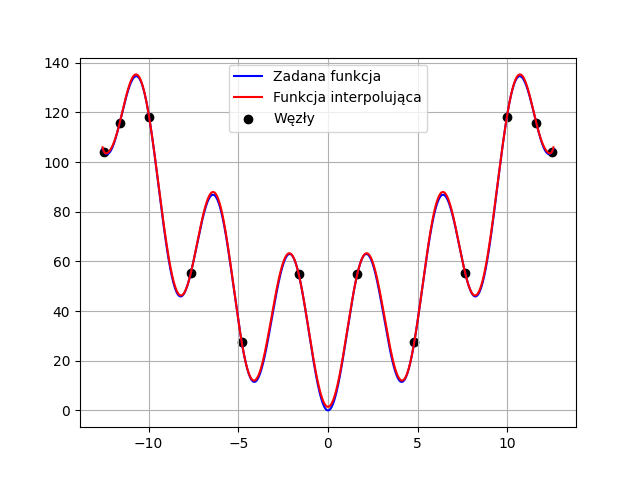
\includegraphics[width=\textwidth]{img06.png}
    \caption{Błąd maksymalny 3-30 dla równoodległych węzłów}
  \end{minipage}
  \hfill
  \begin{minipage}[b]{0.49\textwidth}
    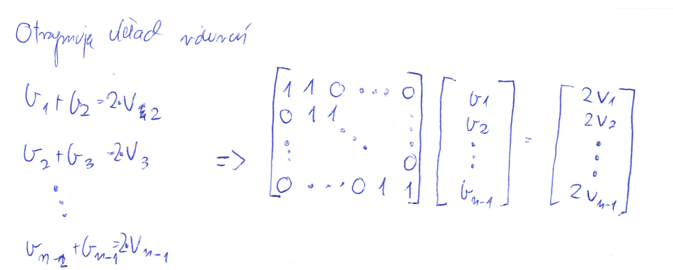
\includegraphics[width=\textwidth]{img07.png}
    \caption{Błąd maksymalny 3-30 dla węzłow Czebyszewa}
  \end{minipage}
\end{figure}

\noindent
W celu sprawdzenia, która metoda przybliżenia jest najlepsza należy spojrzeć na wykres w skali logarytmicznej (wykres 4 i 5).

\begin{figure}[H]
  \begin{minipage}[b]{0.49\textwidth}
    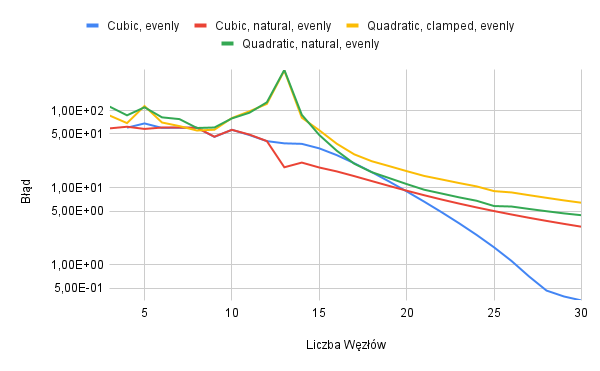
\includegraphics[width=\textwidth]{img18.png}
    \caption{Błąd maksymalny 3-30 dla równoodległych węzłów w skali logarytmicznej}
  \end{minipage}
  \hfill
  \begin{minipage}[b]{0.49\textwidth}
    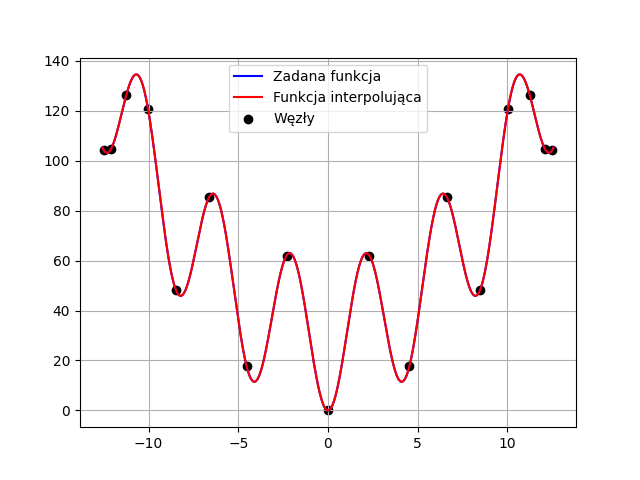
\includegraphics[width=\textwidth]{img19.png}
    \caption{Błąd maksymalny 3-30 dla węzłow Czebyszewa w skali logarytmicznej}
  \end{minipage}
\end{figure}

\noindent
Na podstawie powyższych wykresów można ustalić, że dla węzłów równoodległych z pewnością funkcja sklejana 3-go stopnia jest leprza od funkcji kwadratowej, natomiast jeśli chodzi o warunki brzegowe, jest to dość zmienne w tym przedziale. 
\bigbreak
\noindent
Jeśli chodzi o węzły Czebyszewa sytuacja wygląda podobnie, jednak wartości błedu między różnymi warunkami brzegowymi są bardzo zbliżone, co widać doskonale na wykresie 6.

\begin{figure}[H]
  \begin{minipage}[b]{0.49\textwidth}
    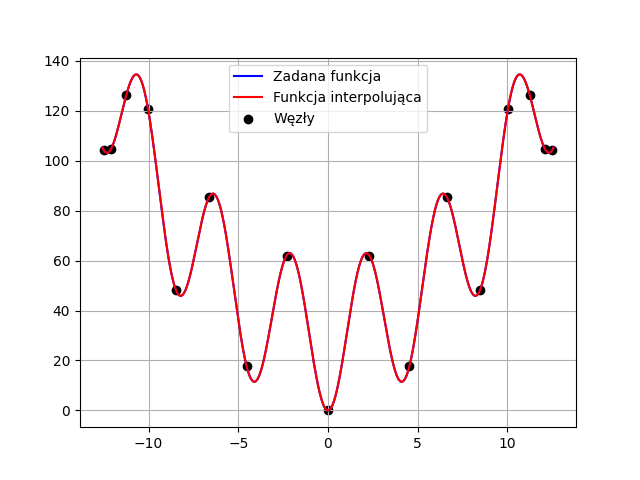
\includegraphics[width=\textwidth]{img20.png}
    \caption{Różnica między funkcją sklejaną 3-go stopnia dla Natural Boundary, a Default Boundary dla funkcji sklejanej 3-go stopnia i węzłów Czebyszewa}
  \end{minipage}
  \hfill
  \begin{minipage}[b]{0.49\textwidth}
    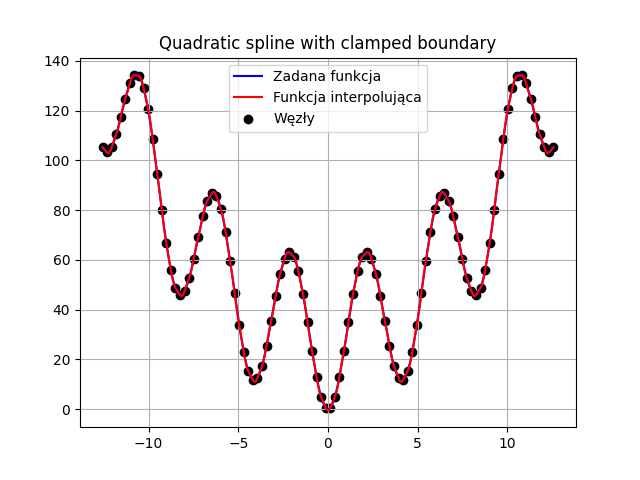
\includegraphics[width=\textwidth]{img22.png}
    \caption{Różnica między funkcją sklejaną 2-go stopnia dla Natural Boundary, a Clamped Boundary dla funkcji sklejanej 3-go stopnia i węzłów Czebyszewa}
  \end{minipage}
\end{figure}


\subsubsection{Błąd maksymalny dla węzłów z zakresu [31, 70]}

Ponownie na wykresach 8 i 9 widać, że wartości otrzymane dla wezłów równoodległych są dużo lepsze niż dla węzłów Czebyszewa, jednak sytuacja wygląda już dużo lepiej dla węzłów Czebyszewa, niż dla przedziału 3-30, gdzie wartości były dość duże.
\bigbreak
\noindent
Patrząc na wykres dla węzłów równoodległych można bardzo ładnie posortować medody przybliżenia funckji. Zatem w kolejności od najlepszej do najgorszej:
\begin{itemize}
\item Funkcja sklejana 3-go stopnia, Default Boundary
\item Funkcja sklejana 3-go stopnia, Natural Boundary
\end{itemize}

A następnie od 31 do 50 węzła:
\begin{itemize}
\item Funkcja sklejana 2-go stopnia, Natural Boundary
\item Funkcja sklejana 2-go stopnia, Clamped Boundary
\end{itemize}

I od 51 do 70 węzła:
\begin{itemize}
\item Funkcja sklejana 2-go stopnia, Clamped Boundary
\item Funkcja sklejana 2-go stopnia, Natural Boundary
\end{itemize}
\bigbreak

Z kolei z uwagi na węzły Czebyszewa:

\begin{itemize}
\item Funkcja sklejana 3-go stopnia, Default Boundary oraz Funkcja sklejana 3-go stopnia, Natural Boundary
\item Funkcja sklejana 2-go stopnia, Clamped Boundary
\item Funkcja sklejana 2-go stopnia, Natural Boundary
\end{itemize}

\noindent
Niestety nawet wartości błędu dla najlepszej metody przybliżenia są dość duże, bo rzędu ok 10E-2.

\begin{figure}[H]
  \begin{minipage}[b]{0.49\textwidth}
    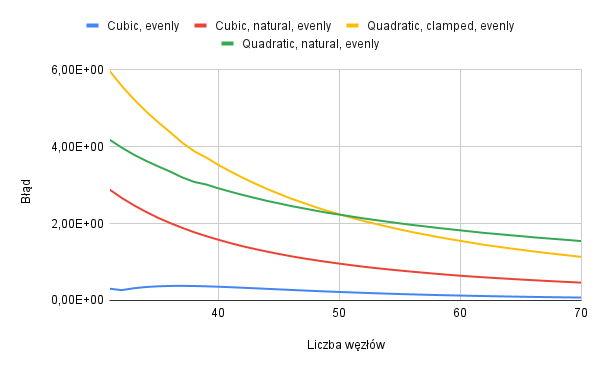
\includegraphics[width=\textwidth]{img08.png}
    \caption{Błąd maksymalny 31-70 dla równoodległych węzłów}
  \end{minipage}
  \hfill
  \begin{minipage}[b]{0.49\textwidth}
    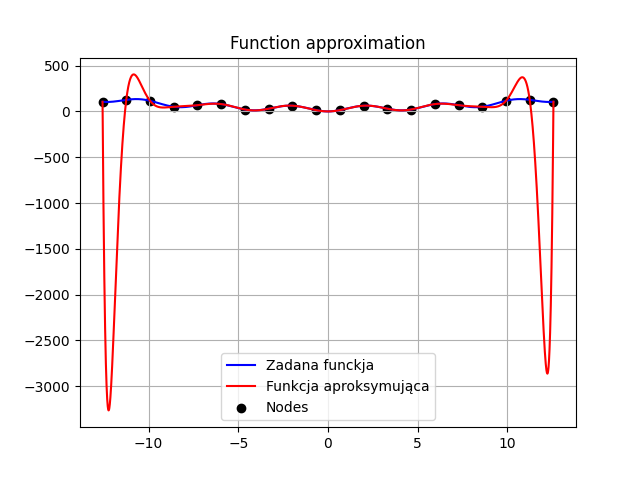
\includegraphics[width=\textwidth]{img09.png}
    \caption{Błąd maksymalny 31-70 dla węzłow Czebyszewa}
  \end{minipage}
\end{figure}

\noindent Tutaj z uwagi na dość liniowe zachowanie wykresów błędów można by pokusić się o zestawienie wszystkich metod przybliżenia, także ze względu na węzły i porównanie ich efektywności (wykres 10), jednak nadal przybliżenie dość mocno zalezy od ilości węzłów i ulega zmianie:

\begin{figure}[H]
  \centering
  \begin{minipage}[b]{0.93\textwidth}
    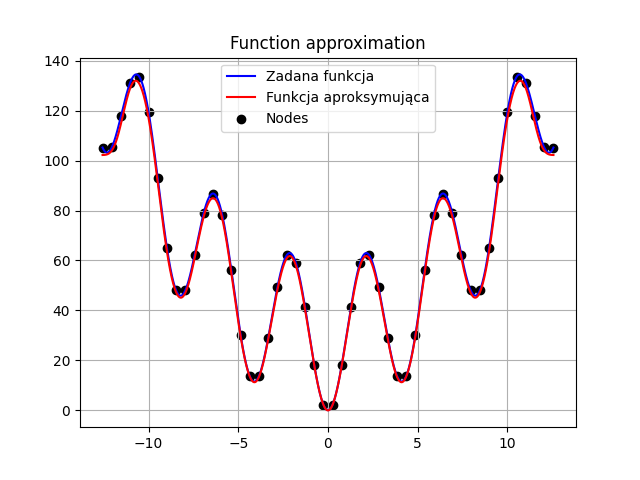
\includegraphics[width=\textwidth]{img24.png}
    \caption{Porównanie efektywności metod przybliżenia w przedziale [31-70]}
  \end{minipage}
\end{figure}

\subsection{Błąd średniokwadratowy}

Identycznie jak w przypadku błędu maksymalnego, błąd został wyliczony dla funkcji sklejanej 2-go i 3-go stopnia oraz różnych warunków brzegowych. Dla każdego wariantu, wybrałem także dwa sposoby generowania węzłów tj. równoodległe oraz Czebyszewa.

\subsubsection{Błąd średniokwadratowy dla węzłów z zakresu [3, 31]}

\bigbreak
Na wykresie dla węzłów równoodległych (wykres 11) błędy są na dość podobnym poziomie, jednak można zaobserwować znaczy peak dla funkcji sklejanej 2-go stopnia przy liczbie 10-15 węzłów. Na wykresie dla węzłów Czebyszewa (wykres 12) sytuacja wygląda gorzej.

\begin{figure}[H]
  \begin{minipage}[b]{0.49\textwidth}
    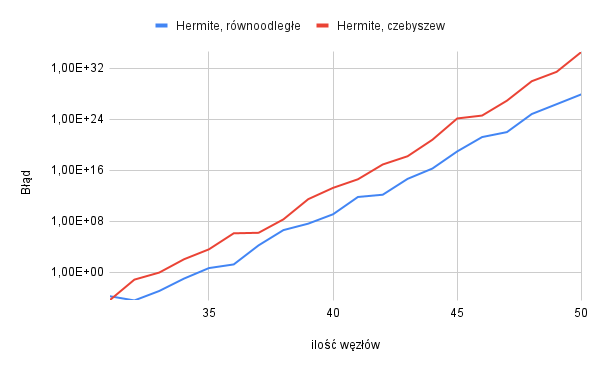
\includegraphics[width=\textwidth]{img10.png}
    \caption{Błąd średniokwadratowy 3-30 dla równoodległych węzłów}
  \end{minipage}
  \hfill
  \begin{minipage}[b]{0.49\textwidth}
    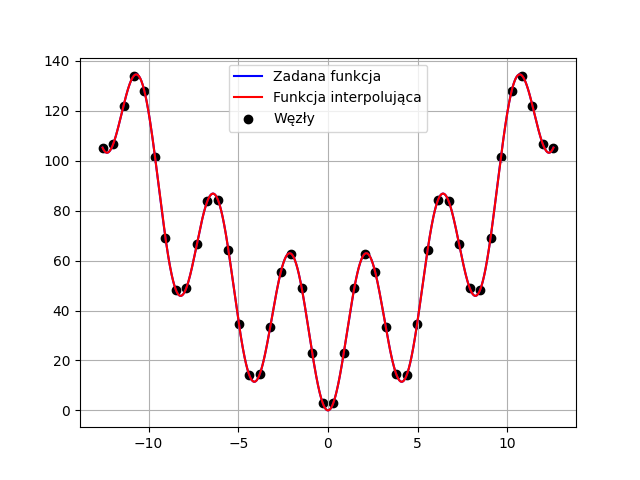
\includegraphics[width=\textwidth]{img11.png}
    \caption{Błąd średniokwadratowy 3-30 dla węzłow Czebyszewa}
  \end{minipage}
\end{figure}

\noindent
Z uwagi na duże podobieństwo wartości błędów zdecydowałem się na wykonanie wykresów w skali logarytmicznej. 

\begin{figure}[H]
  \begin{minipage}[b]{0.49\textwidth}
    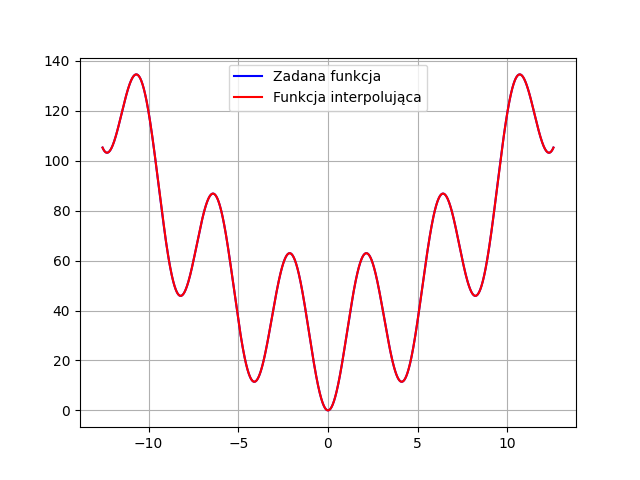
\includegraphics[width=\textwidth]{img12.png}
    \caption{Błąd średniokwadratowy 3-30 dla równoodległych węzłów w skali logarytmicznej}
  \end{minipage}
  \hfill
  \begin{minipage}[b]{0.49\textwidth}
    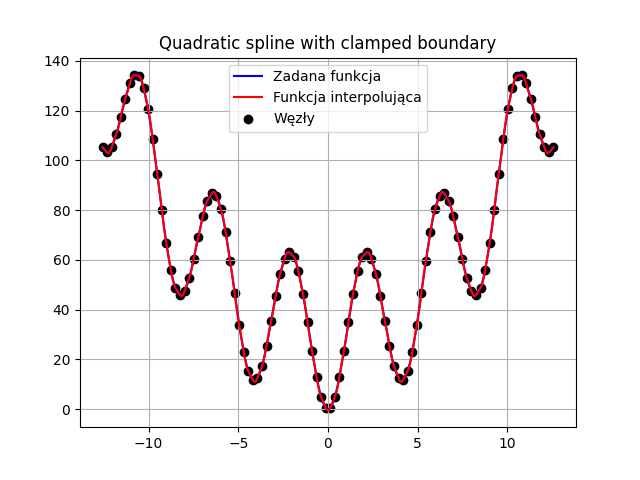
\includegraphics[width=\textwidth]{img21.png}
    \caption{Błąd średniokwadratowy 3-30 dla węzłów Czebyszewa w skali logarytmicznej}
  \end{minipage}
\end{figure}

Na wykresie 13 widać, że dla małej ilości węzłów wartości błędów są bardzo zbliżone. Następnie już od 20 węzła kształtuje się, która metoda przybliżania funkcji jest lepsza. Zatem od 20 do 31 węzłów w kolejności od najlepszej metody do najgorszej:

\begin{itemize}
    \item Funkcja sklejana 3-go stopnia, Default Boundary
    \item Funkcja sklejana 3-go stopnia, Natural Boundary
    \item Funkcja sklejana 2-go stopnia, Natural Boundary
    \item Funkcja sklejana 2-go stopnia, Clamped Boundary
\end{itemize}

\noindent
Jeśli chodzi o węzły Czebyszewa (wykres 14):
\begin{itemize}
\item Funkcja sklejana 3-go stopnia, Default Boundary, Funkcja sklejana 3-go stopnia, Natural Boundary
\item Funkcja sklejana 2-go stopnia, Clamped Boundary
\item Funkcja sklejana 2-go stopnia, Natural Boundary
\end{itemize}

Ze względu na znaczne zbliżenie błędu funkcji sklejanej 3-go stopnie dla dwóch róznych warunków brzegowych, poniżej zamieściłem wykres pokazujący tą różnicę:

\begin{figure}[H]
  \centering
  \begin{minipage}[b]{0.93\textwidth}
    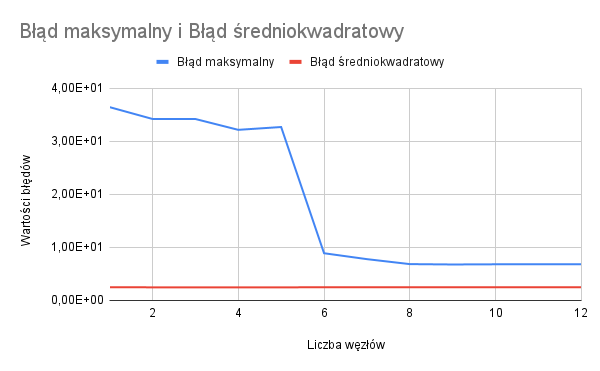
\includegraphics[width=\textwidth]{img23.png}
    \caption{Różnica dla funkcji sklejanej 3-go stopnia i węzłów Czebyszewa oraz Default Boundary i Natural Boundary}
  \end{minipage}
\end{figure}

\noindent
Jak widać na powyższym wykresie 15, wartości są niemal identyczne, duża róznica na początku bierze się stąd, że Defuld Boundary dla 3 węzłów nie istnieje.

\subsubsection{Błąd średniokwadratowy dla węzłów z zakresu [31, 70]}

Jak widać na poniższych wykresach (16 i 17), w tym przedziale dla odmiany węzły Czebyszewa wypadły całkiem dobrze. Tutaj ponownie wartości błędów są dość niskie, jednak dalej nie jest to jakieś bardzo dobre przybliżenie.

\begin{figure}[H]
  \begin{minipage}[b]{0.49\textwidth}
    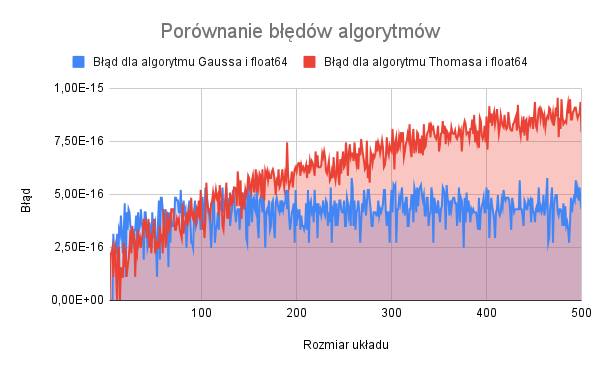
\includegraphics[width=\textwidth]{img13.png}
    \caption{Błąd średniokwadratowy 31-70 dla równoodległych węzłów}
  \end{minipage}
  \hfill
  \begin{minipage}[b]{0.49\textwidth}
    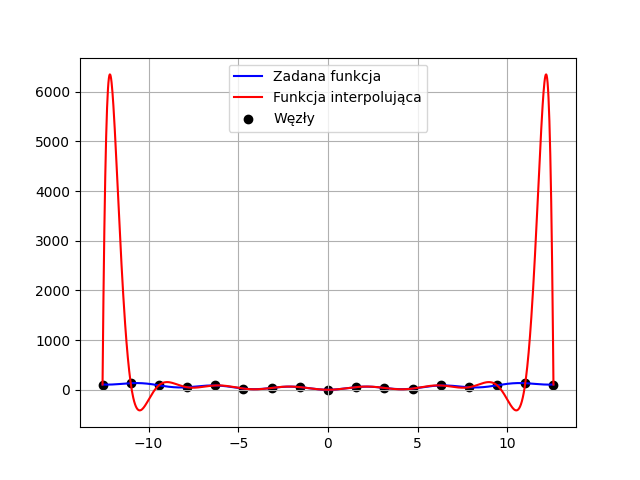
\includegraphics[width=\textwidth]{img14.png}
    \caption{Błąd średniokwadratowy 31-70 dla węzłow Czebyszewa}
  \end{minipage}
\end{figure}

\noindent
Z uwagi na dobry wynik otrzymany dla węzłów Czebyszewa i bliskość błędów otrzymanych dla różnych metod postanowiłem wykonać wykres w sklai logarytmicznej, ale dla wszystkich metod włącznie z różnym sposobem generowania węzłów.


\begin{figure}[H]
  \centering
  \begin{minipage}[b]{0.93\textwidth}
    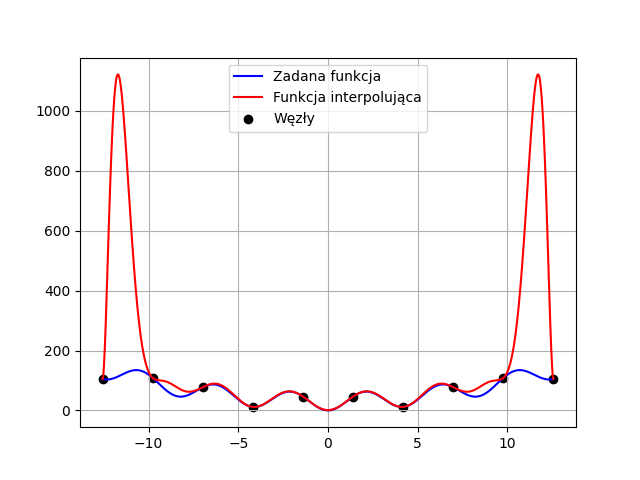
\includegraphics[width=\textwidth]{img15.png}
    \caption{Błąd średniokwadratowy 31-70 w skali logarytmicznej}
  \end{minipage}
\end{figure}

\noindent
Tutaj (wykres 18) już bardzo wyraźnie widać wyższość funkcji sklejanej 3-go stopnia oraz wyższość Default Boundary nad Natural Boundary dla funkcji sklejanej 3-go stopnia. Zatem jeśli chcielibyśmy uszeregować metody przybliżenia od najlepszego do najgorszego w tym przedziale, to dostalibyśmy:

\begin{itemize}
\item Funkcja sklejana 3-go stopnia, Default Boundary, węzły równoodległe
\item Funkcja sklejana 3-go stopnia, Natural Boundary, węzły Czebyszewa, Funkcja sklejana 3-go stopnia, Default Boundary, węzły Czebyszewa
\item Funkcja sklejana 3-go stopnia, Natural Boundary, węzły równoodległe
\item Funkcja sklejana 2-go stopnia, Natural Boundary, węzły Czebyszewa, Funkcja sklejana 2-go stopnia, Clamped Boundary, węzły CZebyszewa
\end{itemize}
Następnie dla węzłów z przedziału [31, 50]
\begin{itemize}
\item Funkcja sklejana 2-go stopnia, Natural Boundary, węzły równoodległe
\item Funkcja sklejana 2-go stopnia, Clamped Boundary, węzły równoodległe
\end{itemize}
Następnie dla węzłów z przedziału [50, 70]
\begin{itemize}
\item Funkcja sklejana 2-go stopnia, Clamped Boundary, węzły równoodległe
\item Funkcja sklejana 2-go stopnia, Natural Boundary, węzły równoodległe
\end{itemize}

\subsection{Porównanie wszystkich metod przybliżenia dla węzłów z zakresu [3, 70]}

Jak widać na wykresach (19 i 20), wysokość błędów znacznie różni się dla różnej ilości węzłów i typów ich generowania. Dlatego, w celu ustalenia najlepszej metody przybliżenia należy zobaczyć jaka metoda dla danej ilości węzłów daje najlepsze rezultaty.

\begin{figure}[H]
  \begin{minipage}[b]{0.49\textwidth}
    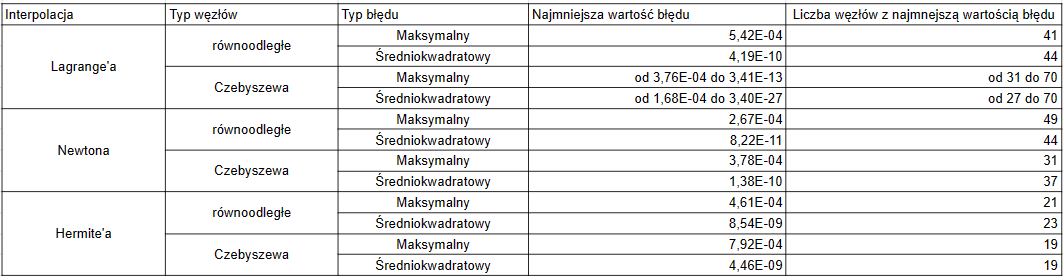
\includegraphics[width=\textwidth]{img16.png}
    \caption{Błąd maksymalny 3-70 dla w skali logarytmicznej}
  \end{minipage}
  \hfill
  \begin{minipage}[b]{0.49\textwidth}
    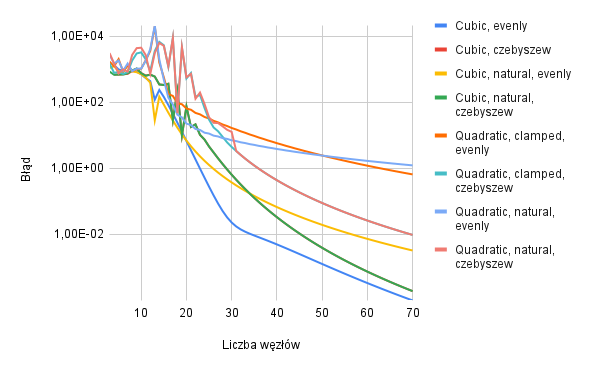
\includegraphics[width=\textwidth]{img17.png}
    \caption{Błąd średniokwadratowy 3-70 w skali logarytmicznej}
  \end{minipage}
\end{figure}

\subsection{Najlepsze przybliżenie}

Bardzo ciężko powiedzieć które przybliżenie jest najlepsze. Napewno można stwierdzić, że ze względu na błąd średniokwadratowy od liczby węzłów >= 20 najelpiej radzi sobie funkcja sklejana 3-go stopnia z równoodległymi węzłami, a przybliżenie uzyskane przez tą funkcję dla 20 (wykres 21) i 70 węzłów wygląda tak:

\begin{figure}[H]
  \begin{minipage}[b]{0.49\textwidth}
    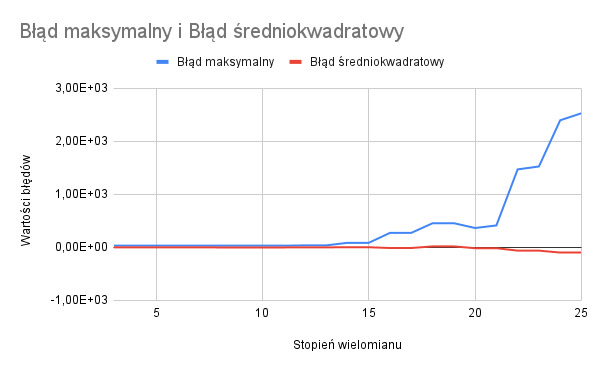
\includegraphics[width=\textwidth]{img25.png}
    \caption{Przybliżenie dla funkcji sklejanej 3-go stopnia i Default Boundary z 20 równoodległymi wezłami}
  \end{minipage}
  \hfill
  \begin{minipage}[b]{0.49\textwidth}
    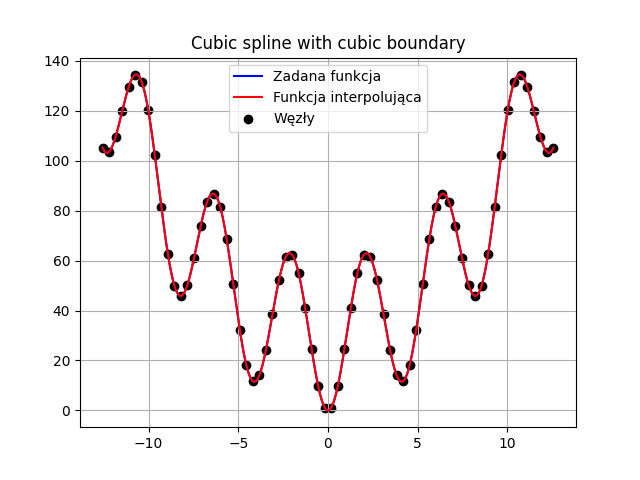
\includegraphics[width=\textwidth]{img26.png}
    \caption{Przybliżenie dla funkcji sklejanej 3-go stopnia i Default Boundary z 70 równoodległymi wezłami}
  \end{minipage}
\end{figure}

\noindent
Można zauważyć, że ze względu na błąd maksymalny w tym przedziale, od ok. 50 węzła lepsze jest przybliżenie dla funkcji sklejanej 3-go stopnia z Natural Boundary i węzłami Czebyszewa.

\bigbreak
\noindent
Natomiast jeśli chodzi o przedział wcześniejszy niż 20 węzłów to jest to bardzo ciężkie do stwierdzenia, która funkcja jest lepsza i bardzo się to zmienia. Napewno z całą pewnością można powiedzieć, że niemal zawsze lepsze przybliżenie otrzymamy dla funkcji sklejanej 3-go stopnia. Tutaj dla prównania poniżej zamieszczam wykres dla 15 węzłów z wykorzystaniem wyranych funkcji sklejanych 2-go i 3-go stopnia:

\begin{figure}[H]
  \begin{minipage}[b]{0.49\textwidth}
    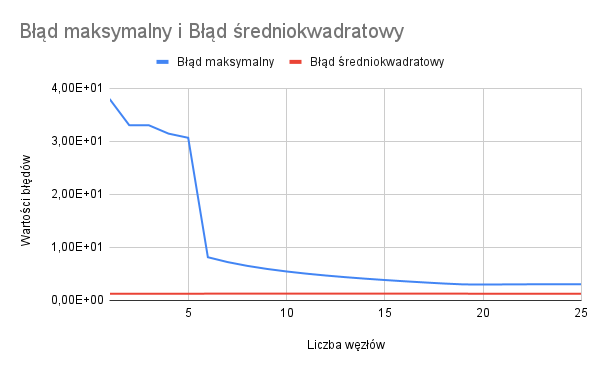
\includegraphics[width=\textwidth]{img28.png}
    \caption{Przybliżenie dla funkcji sklejanej 2-go stopnia i Clamped Boundary z 15 równoodległymi wezłami}
  \end{minipage}
  \hfill
  \begin{minipage}[b]{0.49\textwidth}
    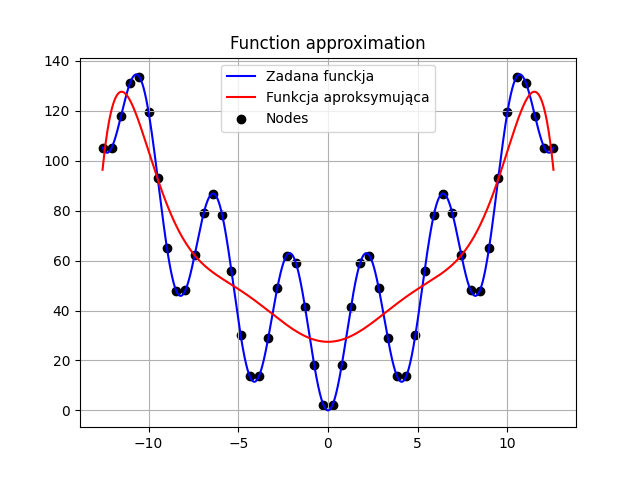
\includegraphics[width=\textwidth]{img29.png}
    \caption{Przybliżenie dla funkcji sklejanej 3-go stopnia i Default Boundary z 15 równoodległymi wezłami}
  \end{minipage}
\end{figure}


\subsection{Wnioski}

\begin{itemize}
\item Dla przedziału [3, 20] węzłów, nie można jasno wskazać, która metoda przybliżenia jest lepsza, ponieważ błąd przybliżenia drastycznie zmienia się w zależności od ilości węzłów
\item Od 20 węzłów w górę najlepsze jest przybliżenie funkcją sklejaną 3-go stopnia z równoodległymi węzłami i Default Boundary
\item Na ogół przybliżenie funkcją sklejaną 3-go stopnia z równoodległymi węzłami i Default Boundary jest najlepsze
\item Na ogół przybliżenie funkcjami sklejanymi 3-go stopnia jest dużo lepsze niż przybliżenie funkcjami sklejanymi 2-go stopnia
\item Przybliżenia otrzymane dla węzłów Czebyszewa, szczegółnie dla małej ilości węzłów są dośc dziwne i często dużo gorsze niż dla węzłów równoodległych
\item Jak bardzo ładnie widać na wykresach zwiększenie liczby węzłów prowadzi do zwiększenia dokładnosci przybliżenia
\end{itemize}

\end{document}
